\section{CƠ SỞ LÝ THUYẾT}\label{sec:co_so_ly_thuyet}

Chương này tóm tắt các khái niệm nền tảng được sử dụng trong thiết kế. Nội dung chi tiết sẽ được trình bày đầy đủ trong báo cáo cuối kỳ.

\subsection{Mạng Campus phân tầng}

Mô hình Core--Distribution--Access chia mạng thành ba tầng có chức năng riêng: tầng Access kết nối thiết bị đầu cuối và gán VLAN; tầng Distribution tập trung lưu lượng, áp chính sách; tầng Core chuyển mạch tốc độ cao và định tuyến giữa các khối. Cách phân tầng giúp khoanh vùng sự cố, dễ mở rộng và tạo điều kiện bố trí dự phòng ở từng tầng (Hình~\ref{fig:core_distribution_access}).

\begin{figure}[H]
    \centering
    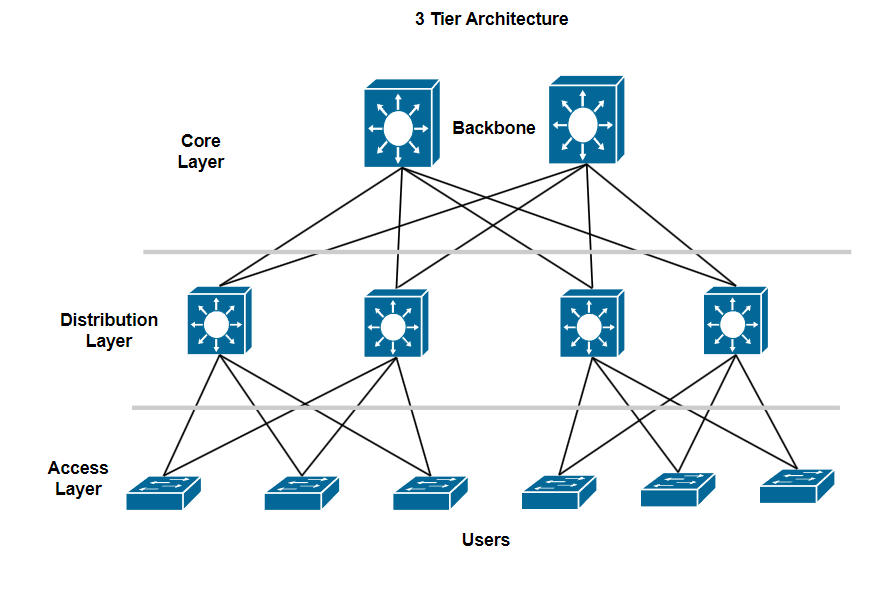
\includegraphics[width=0.70\textwidth]{image/mohinh.png}
    \caption{Mô hình mạng Campus Core--Distribution--Access}
    \label{fig:core_distribution_access}
\end{figure}

\subsection{VLAN, định tuyến và dự phòng gateway}

VLAN chia một hạ tầng lớp 2 thành nhiều miền quảng bá độc lập; các VLAN được mang trên đường trunk 802.1Q (Hình~\ref{fig:vlan}). Định tuyến liên VLAN thực hiện trên switch lớp 3 hoặc firewall. VRRP cho phép hai thiết bị chia sẻ một địa chỉ gateway ảo, để máy trạm không phải đổi gateway khi một thiết bị hỏng. OSPF được dùng để trao đổi tuyến nội bộ trong Campus chính, còn BGP được dùng giữa khách hàng và nhà cung cấp dịch vụ ở mạng truyền tải.

\begin{figure}[H]
    \centering
    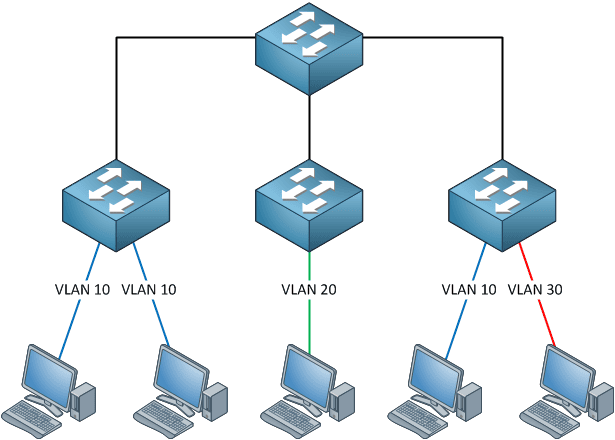
\includegraphics[width=0.65\textwidth]{image/vlan.png}
    \caption{Phân đoạn mạng bằng VLAN}
    \label{fig:vlan}
\end{figure}

\subsection{Software-Defined Networking}

SDN tách mặt phẳng điều khiển (control plane) khỏi mặt phẳng dữ liệu (data plane). Bộ điều khiển tập trung tính toán và cài đặt luật chuyển tiếp (flow) xuống switch qua giao thức southbound như OpenFlow; ứng dụng phía trên tương tác với bộ điều khiển qua API northbound (Hình~\ref{fig:sdn_architecture}).

\begin{figure}[H]
    \centering
    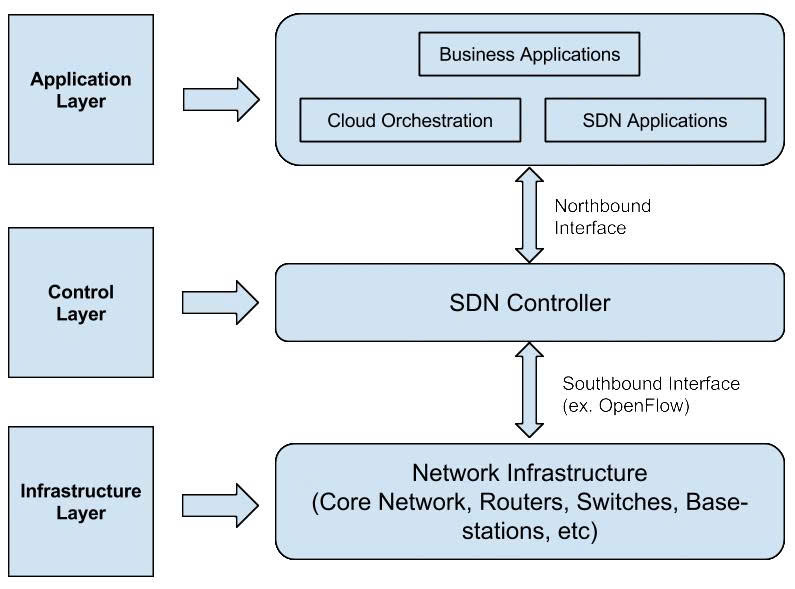
\includegraphics[width=0.55\textwidth]{image/SDN_ARCHITECTURE.jpg}
    \caption{Kiến trúc ba lớp của SDN}
    \label{fig:sdn_architecture}
\end{figure}

Trong OpenFlow 1.3, mỗi switch có các bảng flow gồm trường so khớp, độ ưu tiên và hành động. Gói tin không khớp flow nào sẽ rơi vào luật table-miss, thường được gửi lên bộ điều khiển dưới dạng \texttt{packet-in}. Bộ điều khiển học địa chỉ MAC, quyết định cổng ra và cài flow để các gói sau được chuyển trực tiếp trên switch (Hình~\ref{fig:sdn_hoat_dong}). Đề tài dùng bộ điều khiển Ryu (Python) và Open vSwitch làm switch OpenFlow.

\begin{figure}[H]
    \centering
    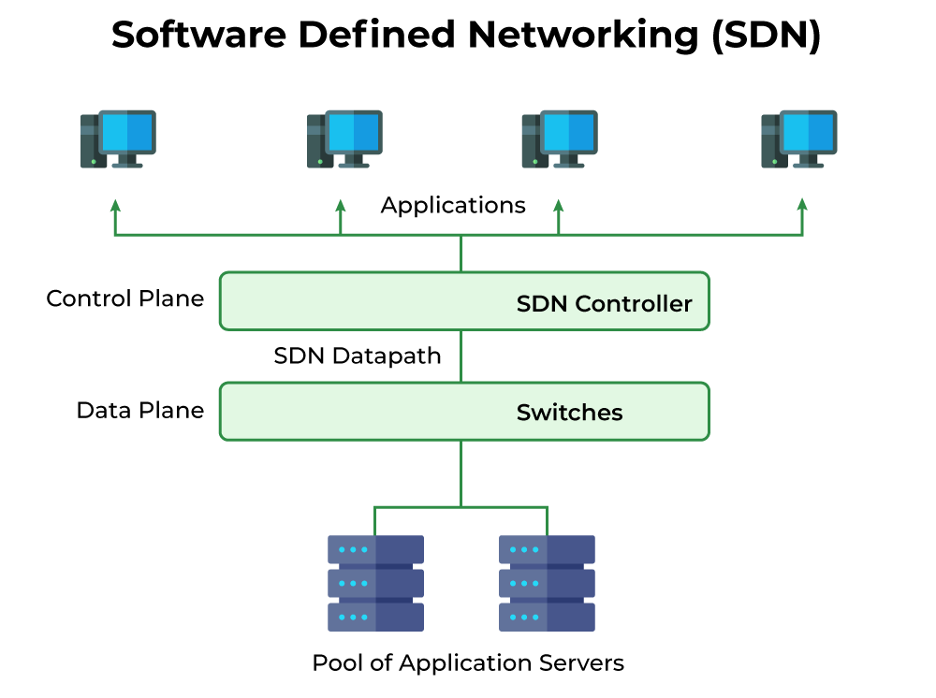
\includegraphics[width=0.70\textwidth]{image/nguyenlyhoatdongsdn.png}
    \caption{Nguyên lý hoạt động của SDN với OpenFlow}
    \label{fig:sdn_hoat_dong}
\end{figure}

\subsection{Software-Defined WAN (Cisco SD-WAN)}

Cisco SD-WAN (Viptela) gồm bốn thành phần (Hình~\ref{fig:sdwan}):

\begin{itemize}
    \item \textbf{vBond (orchestrator):} xác thực thiết bị và điều phối kết nối ban đầu.
    \item \textbf{vManage:} quản lý, cấu hình và giám sát tập trung.
    \item \textbf{vSmart:} bộ điều khiển định tuyến và chính sách, trao đổi tuyến với các edge qua OMP.
    \item \textbf{vEdge:} thiết bị tại site, thiết lập đường hầm IPsec tới các edge khác.
\end{itemize}

\begin{figure}[H]
    \centering
    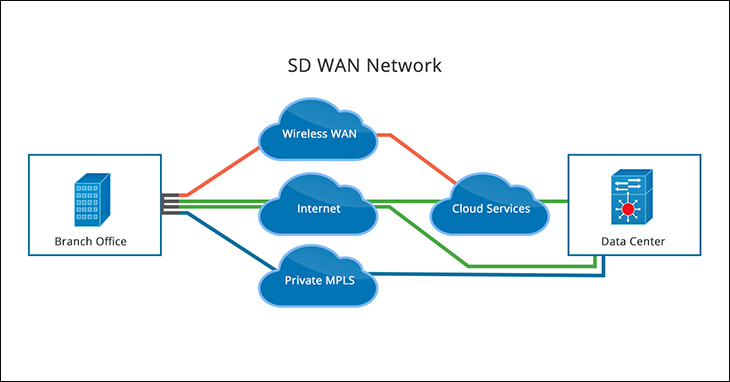
\includegraphics[width=0.70\textwidth]{image/sdwan.jpg}
    \caption{Kiến trúc Cisco SD-WAN}
    \label{fig:sdwan}
\end{figure}

Mỗi điểm kết nối WAN của vEdge là một TLOC, được gắn màu theo loại đường truyền (ví dụ \texttt{biz-internet}, \texttt{mpls}). BFD chạy trong từng đường hầm để phát hiện mất kết nối và đo độ trễ, jitter, tỷ lệ mất gói. Dựa trên số đo này, chính sách Application-Aware Routing chọn đường hầm đáp ứng SLA cho từng loại lưu lượng. Thiết bị chỉ tham gia fabric khi có chứng thư hợp lệ do CA tin cậy ký và có tên trong danh sách thiết bị được phép (whitelist) trên các controller.

\subsection{So sánh mạng truyền thống, SDN và SD-WAN}

SDN và SD-WAN cùng dựa trên nguyên lý tách mặt phẳng điều khiển và điều khiển tập trung, nhưng giải quyết hai bài toán khác nhau: SDN tập trung vào mạng nội bộ, còn SD-WAN tập trung vào kết nối giữa các cơ sở. Bảng~\ref{tab:so_sanh} tóm tắt sự khác biệt giữa ba cách tiếp cận.

\begin{table}[H]
    \centering
    \small
    \caption{So sánh mạng truyền thống, SDN và SD-WAN}
    \label{tab:so_sanh}
    \begin{tabularx}{\textwidth}{|P{2.6cm}|X|X|X|}
        \hline
        \textbf{Tiêu chí} & \textbf{Mạng truyền thống} & \textbf{SDN} & \textbf{SD-WAN} \\
        \hline
        Mặt phẳng điều khiển & Phân tán trên từng thiết bị & Tập trung tại controller & Tập trung tại vSmart \\
        \hline
        Phạm vi áp dụng & LAN và WAN & Chủ yếu LAN, data center & Kết nối WAN giữa các site \\
        \hline
        Cấu hình & Thủ công qua CLI từng thiết bị & Lập trình qua controller & Template, chính sách tập trung trên vManage \\
        \hline
        Giao thức chính & STP, OSPF, BGP & OpenFlow & OMP, BFD, IPsec \\
        \hline
        Chọn đường & Theo metric định tuyến & Theo flow do controller cài & Theo SLA ứng dụng (AAR) \\
        \hline
        Đường truyền & Thường phụ thuộc một nhà cung cấp & Không áp dụng & Nhiều transport (Internet, MPLS, LTE) \\
        \hline
    \end{tabularx}
\end{table}

Trong đề tài, hai công nghệ được kết hợp: SDN quản lý lớp Distribution--Access tại Campus chính, SD-WAN đảm nhận kết nối giữa Campus chính và các chi nhánh, còn firewall và Core vẫn dùng định tuyến truyền thống để làm điểm ghép nối giữa hai miền.
